\chapter{Systém Fitcrack} 
\label{Fitcrack}
\textbf{Fitcrack}~\cite{TR_TARZAN} je distribuovaný systém pre obnovu hesiel šifrovaných médii a prelomenie kryptografických hešov.
Pre samotné lámanie hešov používa Hashcat, ktorý je momentálne najrýchlejšie riešenie na trhu.
Správu hosťov a rozdeľovanie úloh zabezpečuje Berkeley Open Infrastructure framework.
Viac o~týchto nástrojoch obsahuje nasledujúca kapitola.
Vlastné súčasti systému Fitcrack sú ďalej popísané v~\ref{Fitcrack_casti}

\section{Nástroje používané systémom Fitcrack}
Táto kapitola popisuje nástroje poživané systémom Fitcrack.
Ich presné fungovanie je pre testovanie nepodstatné vedieť, ale dôležitá je ich funkcia v~systéme.

\subsection{BOINC}
\label{boinc}
\textit{Berkeley Open Infrastructure for Network Computing} (BOINC)~\cite{boincintro} je platforma pre distribuované výpočty, ktorá natívne podporuje dynamické pripojovanie uzlov cez internet.
BOINC bol primárne vytvorený ako nástroj na verejné zdieľanie výpočtových  prostriedkov v~oblastiach ako je meteorológia, medicína, astrofyzika a ďalšie.
Dobrovoľník môže poskytnúť svoje výpočtové kapacity niektorému z~projektov.
Každý projekt sa zaoberá niečím iným, napríklad projekt \textit{Search for Extraterrestrial Intelligence} (SETI)~\cite{SETI} využíva výpočtový výkon dobrovoľníckych staníc na analyzovanie signálov z~vesmíru a hľadanie mimozemského života.
Tento princíp sa nazýva volunteer computing.
BOINC podporuje aj tzv. grid computing, teda zapojenie množstva počítačov a výpočtových stredísk z~rôznych geografických lokalít.

Boinc funguje na princípe server/klient, kde server predstavuje server projektu ku ktorému sa pripája ľubovoľný počet klientov.
Klient sa môže pripojiť z~rôznych zariadení, na ktorom beží rôzny operačný systém a sú vybavené rôznymi jednotkami, na ktorých ma byť prevádzaný výpočet (CPU, GPU, FPGA).
Server zodpovedá za prideľovanie pracovných úloh klientom, zaisťuje sťahovanie najnovších spustiteľných súborov na klientské zariadenia.
Klient môže byť pripojený na viac projektov a sám si určuje koľko výpočtového výkonu chce poskytnúť na jednotlivé úlohy.
BOINC ráta s~prípadmi, kedy sa klienti pripoja alebo odpoja počas výpočtu a ponúka niekoľko spôsobov riešenia, no konkrétne riešenie je implementované tvorcom projektu.
Keďže je BOINC priamo navrhnutý pre distribuovaný výpočet cez internet ponúka množstvo bezpečnostných mechanizmov na prácu v~nedôveryhodnom prostredí.

\subsection{Hashcat}
\label{hashcat}
\textbf{Hashcat}\footnote{\url{https://hashcat.net/hashcat/}} je svetovo najrýchlejším riešením na lámanie hesiel na jednom stroji.
Je zadarmo, má otvorený zdrojový kód, je spustiteľný na Windowse, Linuxe aj na macOS.
Používa OpenCL, ktoré je už dnes kompatibilné s~väčšinou zariadení ( CPU, GPU, DSP, FPGA, … ) a podporuje množstvo formátov.

\textbf{OpenCL} (Open Computing Language\footnote{\url{https://www.khronos.org/opencl/}}) je štandard pre paralelné programovanie na rôznych typov procesorov používaných v~osobných počítačoch, serveroch, mobilných telefónov a vstavaných systémov.


\section{Vlastné časti systému Fitcrack}
\label{Fitcrack_casti}
Ostatné súčasti sú popísané v~tejto kapitole.
\begin{figure}[H]
\centering
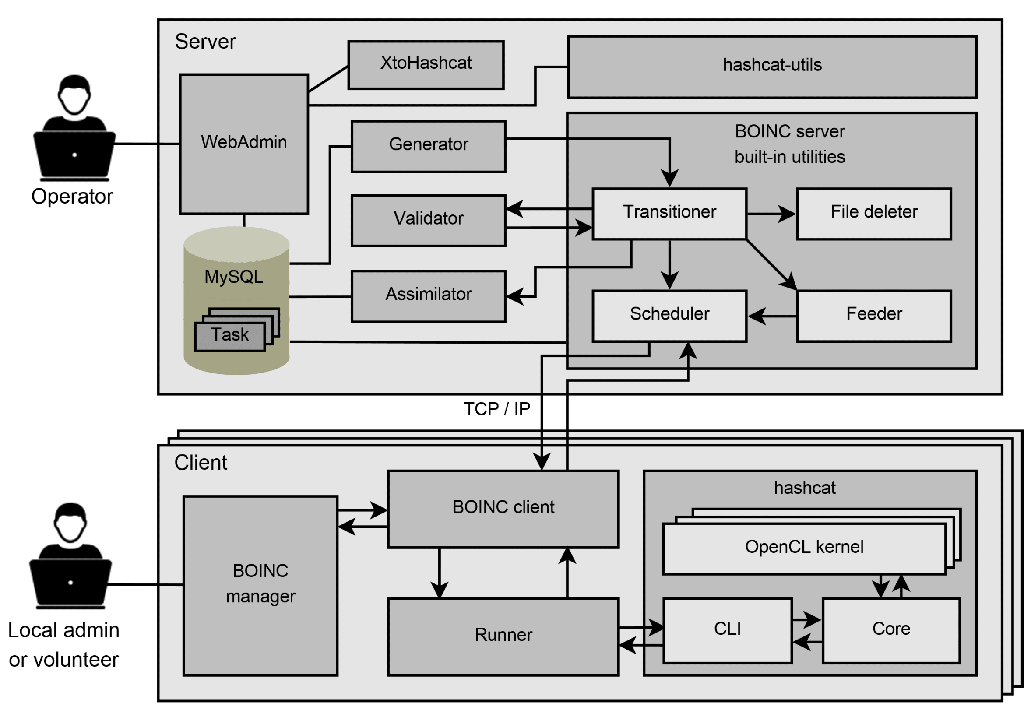
\includegraphics[width=\textwidth]{obrazky/fc_arch-1.png}
\caption{Architektúra systému Fitcrack.~\cite{TR_TARZAN}}
\label{fig:fc_arch}
\end{figure}

BOINC server, BOINC client, BOINC manager a Validator sú súčasti BOINC-u a neboli nijak modifikované.

Je potrebné testovať iba časti systému aspoň čiastočne implementované tvorcami Fitcracku:
\begin{itemize}
	\label{tests_moduls}
	\item \textbf{Generátor},
	\item \textbf{Asimilátor},
	\item \textbf{Runner},
	\item \textbf{XtoHashcat}.
\end{itemize}

\subsection{WebAdmin}
\label{webadmin}
\textbf{WebAdmin} je grafické užívateľské rozhranie pre ovládanie systému Fitcrack a komunikuje s~databázou pomocou REST API, na ktoré sa zameriava študent Matúš Múčka v~svojej budúcej bakalárskej práci.
Testovanie WebAdmina nie je súčasťou tejto práce, keďže práve prebieha vývoj nového grafického užívateľského rozhrania.

\subsection{REST API}
\label{API}
Vyššie spomenuté \textbf{REST API} slúži na komunikáciu GUI a serverových modulov, konkrétne XtoHashcat a Hashcat-utils, čo sú programy podporujúce Hashcat (overovanie formátu hashu, …).
So zbytkom serverových modulov komunikuje cez databázu.
Toto API je schopné vytvárať nové úlohy, sledovať pripojených klientov, mapovať ich na existujúce úlohy, riadiť výpočet úloh, …

\subsection{XtoHashcat}
\label{xtohashcat}
\textbf{XtoHashcat} je skript v~jazyku Python3 vyvinutý tvorcami systému Fitcrack, ktorý dokáže zobrať na vstup ľubovoľný súbor z~množiny podporovaných súborov a na výstup dá heš pre Hashcat.
To znamená, že dokáže detekovať formát súboru a extrahovať heš zo súboru.

\subsection{Generátor}
\label{generator}
\textbf{Generátor}, alebo Work Generator je BOINC server démon bežiaci v~nekonečnom cykle, v~ktorom generuje nové pracovné úlohy(work units) pre pripojených klientov k~danej úlohe(job).
Generátor vytvára 2 typy úloh: benchmark a normálna.
Benchmark úlohy sa generujú klientom, ktorý sa práve pripojili, alebo keď na danom klientovi nastala chyba.
Normálne úlohy sú pracovné úlohy obsahujúce všetky potrebné informácie pre spustenie klientskej časti systému Fitcrack.
Úloha môže byť v~jednom z~nasledujúcich stavov:
\begin{itemize}
	\item \textbf{0 - ready}. Výpočet neprebieha.
	\item \textbf{1 - finished}. Výpočet bol dokončený a heslo nájdené.
	\item \textbf{2 - exhausted}. Výpočet bol dokončený, ale heslo nebolo nájdené.
	\item \textbf{3 - malformed}. Úloha obsahuje chybný vstup.
	\item \textbf{4 - timeout}. Úloha bola ukončená z~dôvodu prekročenia časového limitu.
	\item \textbf{10 - running}. Prebieha výpočet.
	\item \textbf{12 - finishing}. Negenerujú sa nové pracovné úlohy, ale výpočet stále prebieha na niektorých klientských staniciach.
\end{itemize}
V~module Generátor je implementovaný plánovací algoritmus, ktorý vytvára pracovné úlohy na mieru konkrétnej klientskej stanici.
Princíp činnosti modulu Generátor je popísaný algoritmom~\ref{alg:generator}.

\begin{algorithm}[p]
	\caption{Princíp činnosti systemového modulu Generátor}
	\label{alg:generator}
	\DontPrintSemicolon
	\While{1}{
		\tcc{Inicializácia}
		\nlset{0}
		zmaž uzly, ktoré sa podieľajú na riešení úlohy, ktorých pracovný balíček
		je už dokončený, buď úspešne (finished) alebo neúspešne
		(exhausted)\;
		\If{niektorý z~balíčkov presiahol stanovenú dobu ukončenia}{
		\nlset{1}
			nastav jeho stav na finished (12)\;}
		\nlset{2}
		\ForEach{bežiaci pracovný balíček (stav $\geq 10$)}{
			\nlset{3}
			\If{nie je nastavený čas zahájenia}{
				\nlset{4}
				nastáva čas zahájenia na aktuálny čas\;
			}
			\nlset{5}
			\If{k~balíčku sa viažu masky hesiel}{
				\nlset{6}
				ulož ích do príslušného poľa, ktoré odpovedá balíčku\;
			}
			\nlset{7}
			nájdi uzly, ktoré sa majú podieľať na výpočte (a zatiaľ 
			sa nepodieľajú) a ulož ich do databázy\;
			\tcc{Benchmark}
			\nlset{8}
			\ForEach{pridelený aktívny uzol, ktorý ma stav Benchmark (0)}{
				\nlset{9}
				\If{uzol ešte nemá naplánovaný benchmark}{
					\nlset{10}
					naplánuj benchmark pre tento uzol\;
				}
			}
			\tcc{Výpočet}
			\nlset{11}
			\ForEach{aktívny uzol v~stave Normal (1)}{
				\nlset{12}
				\If{počet naplánovaných úloh pre uzol $\geq 2$}{
					\nlset{13}
					pokračuj na ďalší uzol\;
				}
				\nlset{14}
				\If{Stav uzlu je Running (10)}{
					\nlset{15}
					vygeneruj novú úlohu podľa typu balíčka, prípadne
					znovu prideľ nedokončené úlohy\;
				}
				\nlset{16}
				\If{stav uzle je Finished (12)}{
					\nlset{17}
					znovu prideľ nedokončené úlohy, ak taká neexistuje,
					nastav stav uzlu na Done (3)\;
				}
				\tcc{Kontrola stavu}
				\nlset{18}
				\If{stav balíčka je Finished (12) a neobsahuje žiadne úlohy}{
					\nlset{19}
					\eIf{aktuálny čas > plánovaný čas ukončenia}{
						\nlset{20}
						nastav stav balíčka na Timeout (4)\;
					}{
						\nlset{21}
						\eIf{aktuálny index $\geq$ maximálny index}{
							\nlset{22}
							nastav stav balíčku na Exhausted (2)\;
							\tcc{vyčerpaný stavový priestor}
						}{
							\nlset{23}
							nastav stav balíčku na Ready(0)\;
							\tcc{výpočet bol pozastavený}
						}
					}
				}
			}
		}
		\nlset{24}
		čakaj stanovený časový interval\;
	}
\end{algorithm}

\subsection{Asimilátor}
\label{asimilator}
\textbf{Asimilátor} je takisto BOINC server démon, ktorý spracováva valídne výsledky.
Nekonečný cyklus v~ktorom beží je poskytnutý BOINC-om, ale samotná akcia, ktorá sa vykonáva pri prijatí výsledku je implementovaná tvorcami Fitcrack-u.
Funkčnosť akcie je prezentovaná algoritmom~\ref{alg:asimilator}.

\begin{algorithm}[h]
	\caption{Princíp činnosti modulu Asimilátor}
	\label{alg:asimilator}
	\DontPrintSemicolon
	\While{1}{
		\nlset{0}
		\Switch{typ}{
			\Case{benchmark}{
				\nlset{1}
				\eIf{výsledok je v~poriadku (kód 0)}{
					\nlset{2}
					prečítaj zmeraný výkon\;

					\If{mód útoku je mask}{
						\nlset{3}
						preveď prepočet na hashcat-indexy\;
						}
					\nlset{4}
					ulož výkon hosťa do databázy\;
					prečítaj čas benchmarku a ulož do databázy\;
				}{
					\nlset{5}
					naplánuj nový benchmark na dlhší čas\;
				}
			\nlset{6}
			}\Case{normal}{
				\nlset{7}
				\eIf{heslo bol nájdené (kód 0)}{
					\nlset{8}
					prečítaj heslo a ulož ho do databázy (prípadne aj do cache)\;
					uprav stav úlohy na Finished (1)\;
					pošli všetkým zapojeným uzlom pokyn k~ukončeniu výpočtu\;
					odstráň/archivuj nedokončené úlohy\;
					prečítaj časvýpočtu úlohy a ulož ho\;
				}{
					\nlset{9}
					\eIf{heslo nebolo nájdené (kód 1)}{
						\nlset{10}
						prečítaj čas výpočtu a ulož do databázy\;

						\If{úloha mala dostatočnú veľkosť}{
							\nlset{11}
							uprav výkon hosta podľa dĺžky výpočtu poslednej úlohy\;
							}
						\nlset{12}
						pričítaj veľkosť spracovane úlohy k počtu už overených hesiel\;
					}{
						\tcc{Chyba výpočtu}
						\nlset{13}
						zruš všetky bežiace úlohy daného hosta\;
						nastav týmto hostom prínak "retry"\;
						nastav výkon hosta na 0\;
						nastav stav hosta na benchmark (0)\;

						ukonči assimilaciu\;
					}
				}
			}
		}
		
		\nlset{14}
		\eIf{systém je nastavený na mazanie úloh}{
			\nlset{15}
			zmaž položku úlohy z databáze\;
		}{
			\nlset{16}
			nastav položke úlohy príznak "finished"\;
		}
	}
\end{algorithm}

\subsection{Runner}
\label{runner}
\textbf{Runner} je aplikácia bežiaca na klientskom počítači ovládajúca Hashcat.
BOINC server pošle údaje o~pracovnej úlohe BOINC klientovi, ktorý pomocou systémových volaní spúšťa runner a predáva mu tieto informácie v~podobe vstupných súborov.
Runner následne tieto informácie predá nástroju Hashcat.
Runner sleduje stav výpočtu a po je jeho skončení predá výsledky BOINC klientovi.


Generátor a Asimilátor komunikujú výhradne pomocou databázy, kde to validátor a runner riadi priamo BOINC.
Okrem BOINC klienta nie je potrebné na klientskom zariadení nič inštalovať, BOINC klient sám zo servera sťahuje najnovšie spustiteľné súbory v~závislosti na architektúra klientského zariadenia.

\todo{TLV slovník}
\begin{figure}[H]
	\centering
	
\includegraphics[width=\textwidth]{obrazky/keep-calm.png}
	\caption{Schéma komunikácie.}
\end{figure}
\todo{obrázok generátor -> TLV -> runner -> out -> assimilátor}

